% siminos/atlas/slice.tex  pdflatex atlas
% $Author$ $Date$


\section{Slices}
% Reduction of continuous symmetry
\label{s:slice}

The goal of \emph{symmetry reduction} is to replace each group orbit by a
unique point in a lower-dimensional symmetry-\reducedsp\ $\pSRed =
\pS/\Group$, as sketched in \reffig{fig:BeThTraj}.
    \PC{replace the term `symmetry reduction' by a term that does not
    (1) does not imply `reduction' (2) does not conflict with Lie theory
    and gen. relativity meaning of the term
    }

%%%%%%%%%%%%%%%%%%%%%%%%%%%%%%%%%%%%%%%%%%%%%%%%%
% 2011-08-23 Predrag: replaces BeThTraj.pdf from
% dasbuch/book/FigSrc/inkscape/BeThTraj.svg
% 2011-09-09 Predrag: updated
%            continuous.tex overheads, and ChaosBook
\begin{figure}
 \begin{center}
  \setlength{\unitlength}{0.20\textwidth}
  %% \unitlength = units used in the Picture Environment
(a)~~
  \begin{picture}(1,1.07471658)%
    \put(0,0){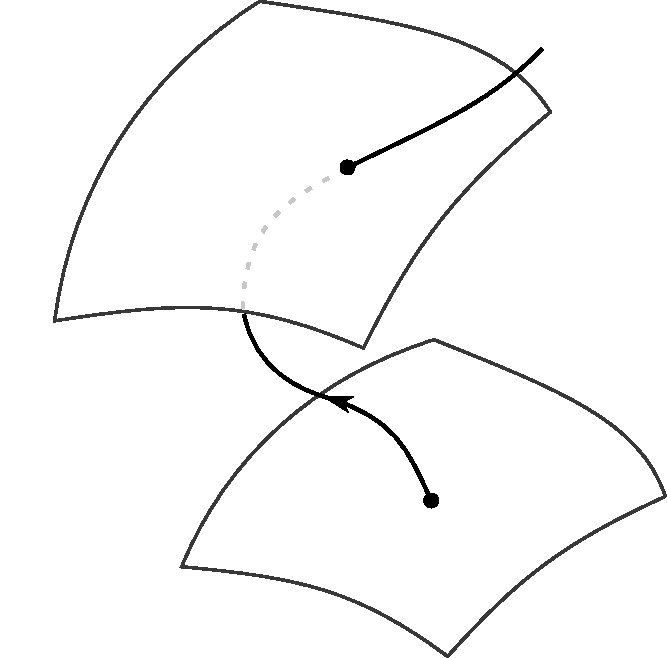
\includegraphics[width=\unitlength]{BeThTrajTeX}}%
    \put(0.28879298,1.02196543){\color[rgb]{0,0,0}\rotatebox{-22.37140782}{\makebox(0,0)[lb]{\smash{$\pS_{\ssp(\zeit)}$}}}}%
    \put(0.55566402,0.45078735){\color[rgb]{0,0,0}\rotatebox{-16.6673442}{\makebox(0,0)[lb]{\smash{$\pS_{\ssp(0)}$}}}}%
    \put(0.63028127,0.18433597){\color[rgb]{0,0,0}\rotatebox{0.03136739}{\makebox(0,0)[lb]{\smash{$\ssp(0)$}}}}%
    \put(0.46253394,0.70182304){\color[rgb]{0,0,0}\rotatebox{0.03136739}{\makebox(0,0)[lb]{\smash{$\ssp(\zeit)$}}}}%
    \put(0.03852492,0.09250899){\color[rgb]{0,0,0}\rotatebox{0.11031334}{\makebox(0,0)[lb]{\smash{$\pS$}}}}%
  \end{picture}%
~~(b)
  \begin{picture}(1,1.07315413)%
    \put(0,0){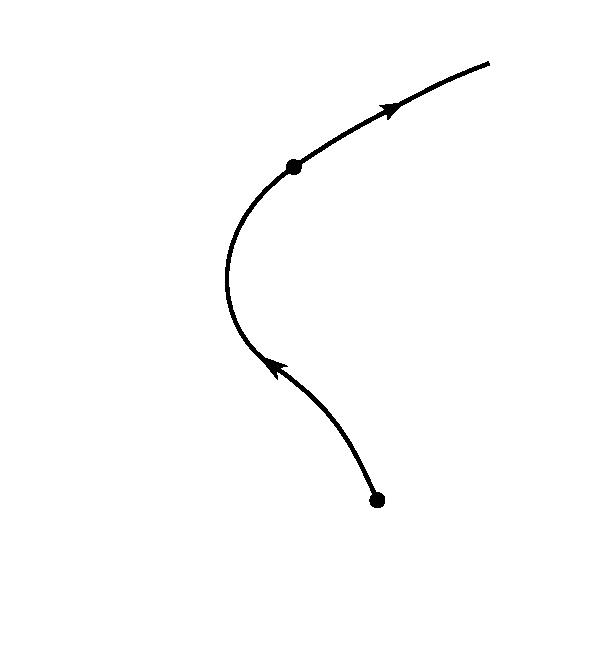
\includegraphics[width=\unitlength]{BeThRedTeX}}%
    \put(0.19912369,0.17144733){\color[rgb]{0,0,0}\rotatebox{0.11031334}{\makebox(0,0)[lb]{\smash{$\pSRed$}}}}%
    \put(0.63028127,0.18433598){\color[rgb]{0,0,0}\rotatebox{0.03136739}{\makebox(0,0)[lb]{\smash{$\sspRed(0)$}}}}%
    \put(0.46253394,0.70182305){\color[rgb]{0,0,0}\rotatebox{0.03136739}{\makebox(0,0)[lb]{\smash{$\sspRed(\zeit)$}}}}%
  \end{picture}%
 \end{center}
% (a) 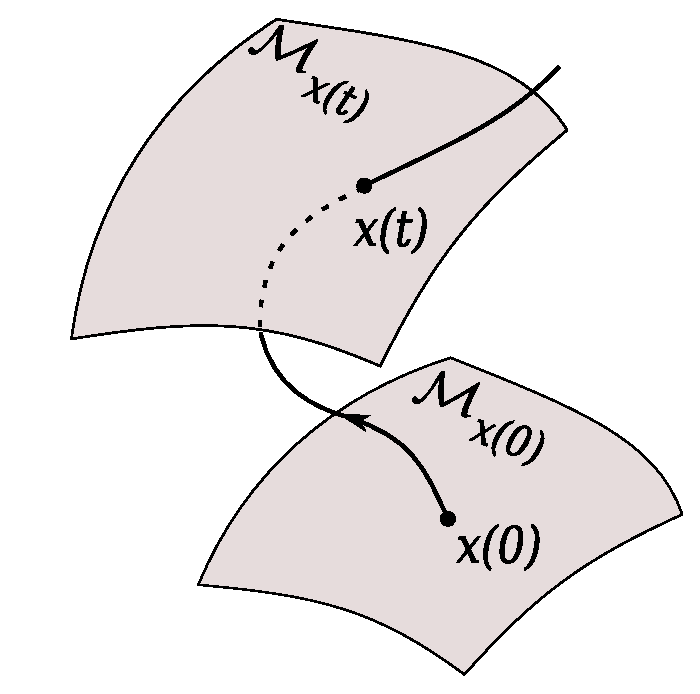
\includegraphics[width=0.45\textwidth]{BeThTraj}
  \caption{\label{fig:BeThTraj}
(a)
The group orbit $\pS_{\ssp(0)}$ of \statesp\ point $\ssp(0)$, and the
group orbit $\pS_{\ssp(\zeit)}$ reached by the trajectory $\ssp(\zeit)$ time $t$
later.
(b)
Symmetry reduction $\pS \to \pSRed$ replaces $\pS_{\ssp}\subset\pS$ by a
single point $\sspRed \in \pSRed$.
  }
\end{figure}
%%%%%%%%%%%%%%%%%%%%%%%%%%%%%%%%%%%%%%%%%%%%%%%%%%

What is a smart way to go about it? Pipe flow intuition,
\reffig{fig:A27-pipeSymms}, might again be helpful. A turbulent flow
exhibits a myriad of unstable structures, all speeding down the pipe,
each with its own {\phaseVel}. The
\mslices\rf{rowley_reconstruction_2000,BeTh04,SiCvi10,FrCv11} tells you
how to pull each solution back into a {\em fixed} frame, the \slice, and
there compare it to your repertoire of precomputed solutions, the
\template s $\{\slicep{}^{(j)}\}$, by a very geometrical idea, the
closest distance to each. What follows is very much like the the
\refsect{s:cut}; due to the linear action of the symmetry group, slicing
is easier than sectioning, but is wholly unfamiliar - that is why we
warmed up by reviewing the Poincar\'e sections.

Symmetries of the flow (i.e.\ the transformations $\LieEl\in\Group$) are
then used to shift and rotate the {\template} $\slicep$ until it
overlies, as well as possible, the state $\ssp$, by minimizing the
distance
\beq
\Norm{\ssp - \LieEl(\gSpace)\,\slicep}
\, .
\ee{minDistance}
The entire group orbit of $\ssp$ is then replaced by the closest match to
the template pattern, given by $\sspRed=\LieEl^{-1}\ssp$. The
symmetry-\reducedsp\ $\pSRed$ (hereafter referred to as the `slice'), of
dimension $(d\!-\!1)$, consists of the set of closest matches $\sspRed$,
one element for each full \statesp\ $\pS$ group orbit; the hat on
$\sspRed$ indicates the unique point on the group orbit of $\ssp$ closest
to the \template\ \slicep.

%%%%%%%%%%%%%%%%%%%%%%%%%%%%%%%%%%%%%%%%%%%%%%%%%%%%%%%%%%%%%%%%%%%%%
\begin{figure}[h]
	\begin{center}
  	\setlength{\unitlength}{0.25\textwidth}
  	\begin{picture}(1,0.62007592)%
    	\put(0,0){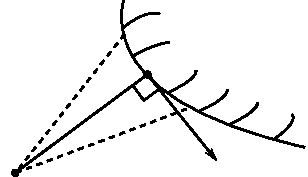
\includegraphics[width=\unitlength]{A28extremum2}}%
    	\put(0.8274739,0.27313042){\color[rgb]{0,0,0}\makebox(0,0)[lb]{\smash{$\LieEl\,\ssp$}}}%
    	\put(0.71822871,0.05712263){\color[rgb]{0,0,0}\makebox(0,0)[lb]{\smash{$\sliceTan{}$}}}%
    	\put(-0.00055527,0.03229441){\color[rgb]{0,0,0}\makebox(0,0)[lb]{\smash{$\slicep$}}}%
    	\put(0.50966967,0.33520145){\color[rgb]{0,0,0}\makebox(0,0)[lb]{\smash{$\sspRed$}}}%
  	\end{picture}
  \end{center}
  \caption{\label{fig:A28extremum}
  Extremal condition \refeq{PCsectQ0} for the point $\sspRed$ on the
  $\ssp$ group orbit that is nearest to the \template\ $\slicep$.
  }
\end{figure}
%%%%%%%%%%%%%%%%%%%%%%%%%%%%%%%%%%%%%%%%%%%%%%%%%%%%%%%%%%%%%%%%%%%%%


For the reduction of a $\SOn{2}$ symmetry, the minimal distance satisfies
the extremum condition (\reffig{fig:A28extremum})
\[
\frac{\partial}{\partial \gSpace} \Norm{\ssp - \LieEl(\gSpace)\,\slicep}^2
   =
2\, \braket{\sspRed - \slicep}{\sliceTan{}}
   = 0
        \,,\quad
\sliceTan{} = \Lg \slicep
\,.
\]
$\Norm{\LieEl(\gSpace)\slicep}$ is a constant, the group tangent vector
$\sliceTan{}$ evaluated at $\slicep$ \refeq{eq:tang} is normal to
$\slicep$, and the term $\braket{\slicep}{\Lg \,\slicep}$ vanishes ($\Lg$
is antisymmetric). Therefore  $\sspRed$, the point on the group orbit that
lands in the \slice, satisfies the \emph{\slice\ condition}
\beq
\braket{\sspRed}{\sliceTan{}} = 0
    \,.
\ee{PCsectQ0}
The \slice\ so defined is thus a hyperplane normal to the \template\
group tangent evaluated at the \template.

Conversely, a template has to be equivariant under infinitesimal actions
of the symmetry group in order that the slice is of dimensionality
$(d-N)$. The {\template} $\slicep$
should be a generic \statesp\ point in the sense that its group orbit has
the full $N$ dimensions of the group \Group. The set of the group orbit
points \emph{closest} to the \template\ \slicep\ form an open connected
neighborhood of \slicep, a neighborhood in which each group orbit
intersects the hyperplane \emph{only once}. This neighborhood is
contained in a half-hyperplane, bounded on one side by the intersection
of the hyperplane section with its {\chartBord}.

We refer to this connected open neighborhood
of \slicep\ as a \emph{chart} $\pSRed_{\slicep} \supset \pS/\Group$,
and
to  \refeq{PCsectQ0} as the \emph{slice conditions}.

%%%%%%%%%%%%%%%%%%%%%%%%%%%%%%%%%%%%%%%%%%%%%%%%%%%%%%%%%%%%%%%%
%% slice.*, inflectHype.*: see dasbuch/book/FigSrc/inkscape/00ReadMe.txt
%% rpo.* hand-drawn in dasbuch/book/FigSrc/xfig/rpo.fig
%% xfig exported -> FigSrc/inkscape/rpo.fig
%% inkscape exported -> rpo.eps + LaTeX, hand edited in the macros
%% Predrag 2011-08-27 replaced rpo.pdf by rpoSlice.pdf
%% remember to insert rpoSlice.pdf into ChaosBook

 \begin{figure}
 \begin{center}
  \setlength{\unitlength}{0.40\textwidth}
  %% \unitlength = units used in the Picture Environment
(a)
  \begin{picture}(1,0.87085079)%
    \put(0,0){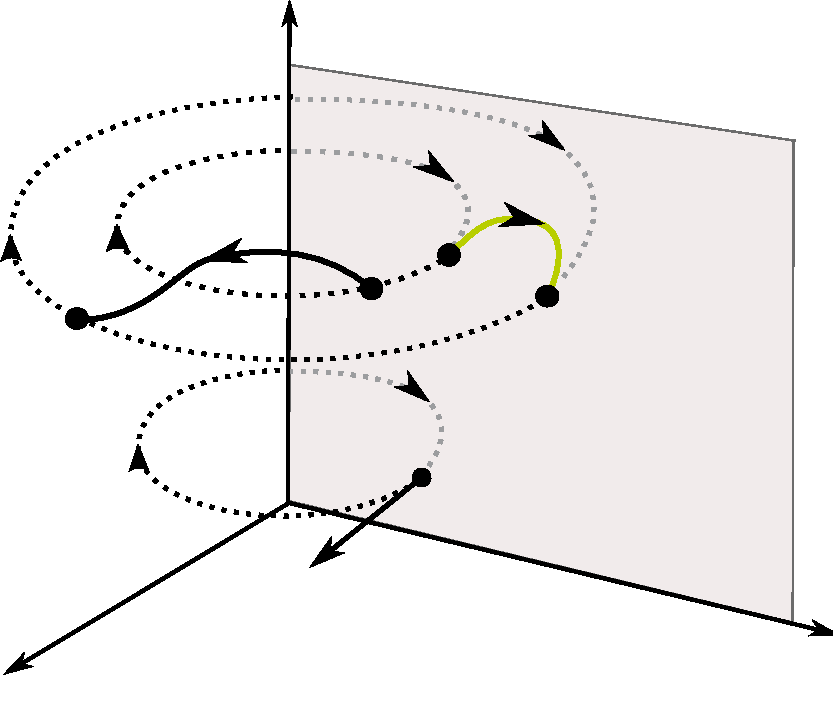
\includegraphics[width=\unitlength]{slice}}%
    \put(0.82835155,0.19007659){\color[rgb]{0,0,0}\rotatebox{-14.84025424}{\makebox(0,0)[lb]{\smash{$\pSRed$}}}}%
    \put(0.07077338,0.28688228){\color[rgb]{0,0,0}\rotatebox{0.0313674}{\makebox(0,0)[lb]{\smash{$\LieEl\,\slicep$}}}}%
    \put(0.53023327,0.26593335){\color[rgb]{0,0,0}\rotatebox{0.0313674}{\makebox(0,0)[lb]{\smash{$\slicep$}}}}%
    \put(0.4284954,0.179285){\color[rgb]{0,0,0}\rotatebox{0.0313674}{\makebox(0,0)[lb]{\smash{$\sliceTan{}$}}}}%
    \put(0.00798985,0.42305068){\color[rgb]{0,0,0}\rotatebox{0.0313674}{\makebox(0,0)[lb]{\smash{$\ssp(\zeit)$}}}}%
    \put(0.65766235,0.45412105){\color[rgb]{0,0,0}\rotatebox{0.0313674}{\makebox(0,0)[lb]{\smash{$\sspRed(\zeit)$}}}}%
    \put(0.06916446,0.74280851){\color[rgb]{0,0,0}\rotatebox{0.0313674}{\makebox(0,0)[lb]{\smash{$\LieEl(\zeit)$}}}}%
  \end{picture}%
\\ %~~~
(b)
  \begin{picture}(1,0.87085079)%
    \put(0,0){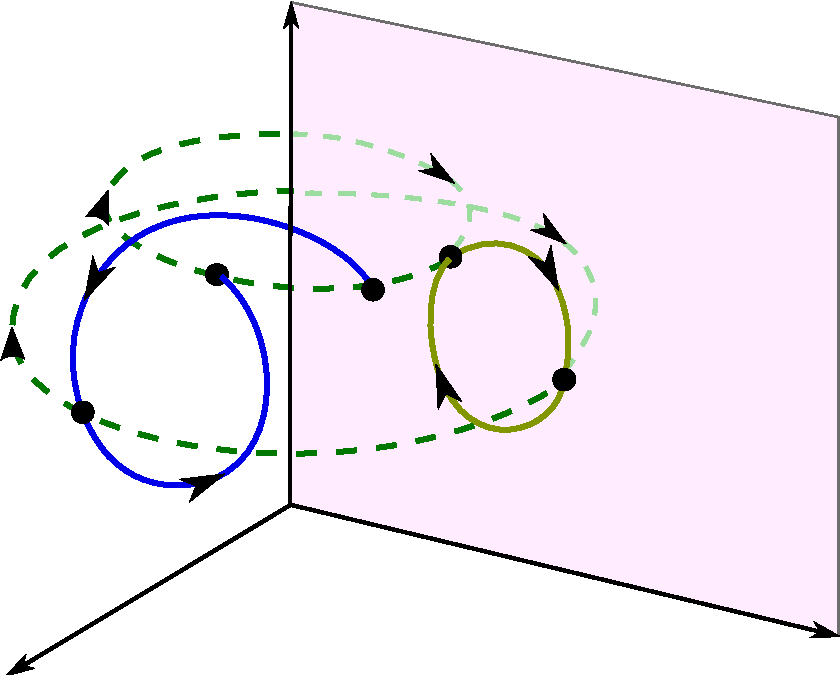
\includegraphics[width=\unitlength]{rpoSlice}}%
    \put(0.82835153,0.19007656){\color[rgb]{0,0,0}\rotatebox{-14.84025432}{\makebox(0,0)[lb]{$\pSRed$}}}%
    \put(0.40925459,0.45713857){\color[rgb]{0,0,0}\rotatebox{0.0313674}{\makebox(0,0)[lb]{\smash{$\ssp(0)$}}}}%
    \put(0.71354118,0.39765314){\color[rgb]{0,0,0}\rotatebox{0.0313674}{\makebox(0,0)[lb]{\smash{$\sspRed(\zeit)$}}}}%
    \put(0.13171187,0.38813817){\color[rgb]{0,0,0}\rotatebox{0.0313674}{\makebox(0,0)[lb]{\smash{$\LieEl(\zeit)$}}}}%
    \put(0.02168739,0.31359574){\color[rgb]{0,0,0}\rotatebox{0.0313674}{\makebox(0,0)[lb]{\smash{$\ssp(\zeit)$}}}}%
    \put(0.15576193,0.48769256){\color[rgb]{0,0,0}\rotatebox{0.0313674}{\makebox(0,0)[lb]{\smash{$\ssp(\period{})$}}}}%
    \put(0.54113911,0.50476963){\color[rgb]{0,0,0}\rotatebox{0.0313674}{\makebox(0,0)[lb]{\smash{$\sspRed(0)$}}}}%
  \end{picture}%
 \end{center}
 \caption{\label{fig:slice}
The \mslices, a \statesp\ visualization:
(a)
\Slice\ $\pSRed \supset \pS/\Group$ lies in the $(d\!-\!N)$\dmn\
hyperplane \refeq{PCsectQ0} normal to $\sliceTan{}$, where $\sliceTan{j}$
span the  $N$\dmn\ space tangent to the group orbit $\LieEl\,\slicep$
(dotted line) evaluated at the {\template} point $\slicep$. The
hyperplane intersects {all} full \statesp\ group orbits (green
dashes).  The full \statesp\
trajectory $\ssp(\zeit)$ (blue) and the \reducedsp\ trajectory
$\sspRed(\zeit)$ (green) are equivalent up to a `moving frame' rotation
$\ssp(\zeit)=\LieEl(\zeit)\,\sspRed(\zeit)$, where $\LieEl(\zeit)$ is a
shorthand for $\LieEl(\gSpace(\zeit))$.
(b)
In the full \statesp\ a \rpo\ $\ssp(0) \to \ssp(\zeit) \to
\ssp(\period{})$ returns to the group orbit of $\ssp(0)$ after time
$\period{}$ and a rotation by $\LieEl$,  $\ssp(0)=\LieEl \, \ssp
(\period{})$. A generic \rpo\ fills out quasi-\-periodically what is
topologically a torus (\reffig{fig:CLf01group}\,(b)). In the \slice\ $\pSRed$
the symmetry-reduced trajectory is periodic, $\sspRed(0) =
\sspRed(\period{})$.
 }
 \end{figure}

\refFig{fig:slice} is a highly idealized sketch: A group orbit is a $N$\dmn\
manifold, and even for $\SOn{2}$ it is usually only topologically a
circle, and can intersect a hyperplane
any number of times  (see \reffigs{fig:sliceimage}{fig:chartBord}).

When $\ssp$ is varies in time, $\dot{\ssp}=\vel(\ssp)$, the {\template}
$\slicep$ tracks the motion using the slice condition \refeq{PCsectQ0} to
minimize $\Norm{\ssp(\zeit)-\LieEl(\theta(\zeit))\slicep}$, and the
full-space trajectory $\ssp(\zeit)$ is thus rotated into the
{\reducedsp}, $\sspRed(\zeit) = \LieEl^{-1}\,\ssp(\zeit)$, by appropriate
\emph{moving frame} angles $\{\gSpace(\zeit)\}$, as depicted in
\reffig{fig:slice}\,{(a)}. Specializing to $\SOn{2}$, one can write
the equations for the \reducedsp\ flow, $\dot{\sspRed} =
\velRed(\sspRed)$, confined to the \slice, $\sspRed(\zeit) \in \pSRed$,
as
\bea
\velRed(\sspRed) &=& \vel(\sspRed)
     \,-\, \dot{\gSpace}(\sspRed) \, \groupTan(\sspRed)
\label{EqMotMFrame}\\
\dot{\gSpace}(\sspRed) &=& \braket{\vel(\sspRed)}{\sliceTan{}}
                       /\braket{\groupTan(\sspRed)}{\sliceTan{}}
\,.
\label{reconstrEq}
\eea
In other words, $\vel$, the velocity in the full \statesp, can be written
as the sum of $\velRed$, the velocity component in the \slice, and
$\dot{\gSpace}\,\groupTan$,
the velocity component within the group tangent space. The
$\dot{\gSpace}$ equation is called the {\em reconstruction equation}, as
its integral keeps track of the group shift in the full \statesp.
